\documentclass[tikz,border=6pt]{standalone}
\usepackage{pgfplots}
\pgfplotsset{compat=1.18}
\usepgfplotslibrary{colormaps}
\usetikzlibrary{arrows.meta,decorations.pathreplacing,calc}

\usepackage{amssymb,amsmath,mathtools}
\usepackage[T1]{fontenc}
\usepackage[utf8]{inputenc}
\usepackage{newpxtext,newpxmath}
\usepackage{sectsty}

\usepackage{physics}

\renewcommand{\Re}{\mathrm{Re}}
\renewcommand{\Im}{\mathrm{Im}}

\begin{document}
% ---------- knobs ----------
\def\gridmin{-2}
\def\gridmax{2}
\def\step{0.8}
\def\base{0.35}      % base arrow length multiplier
\def\maxlen{0.6}     % clamp arrows so they don't explode

% Draw helper: arrow at (x,y) with polar (len, ang) after clamping.
\newcommand{\arrowAt}[3]{%
	% #1 = x,y coordinate as TikZ point; #2 = length; #3 = angle in degrees
	\pgfmathsetmacro{\Lraw}{#2}
	\pgfmathsetmacro{\L}{min(\Lraw,\maxlen)}
	\draw[-{Latex[length=2.2mm]}, line width=0.35pt]
	#1 -- ($#1 + (\L*cos(#3), \L*sin(#3))$);
}

% Panel title macro
\newcommand{\ptitle}[1]{\node[align=center] at (0,2.7) {\large #1};}

% Axis macro
\newcommand{\axes}{%
	\draw[->,gray!70] (-2.6,0) -- (2.6,0) node[below right] {$\Re z$};
	\draw[->,gray!70] (0,-2.6) -- (0,2.6) node[above left] {$\Im z$};
	\foreach \t in {-2,-1,1,2} {
		\draw[gray!40] (\t,-2.6) -- (\t,2.6);
		\draw[gray!40] (-2.6,\t) -- (2.6,\t);
	}
}

 ============================================================
 Panel A: omega = dz
 ============================================================
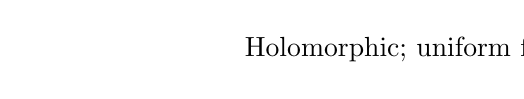
\begin{tikzpicture}[scale=1.0]
	\ptitle{$\omega = dz \quad (f(z)\equiv 1)$}
	\axes
	% Same arrow everywhere: length=base, angle=0
	\foreach \x in {-2,-1.2,-0.4,0.4,1.2,2} {
		\foreach \y in {-2,-1.2,-0.4,0.4,1.2,2} {
			\arrowAt{(\x,\y)}{\base}{0}
		}
	}
	\node[align=left,anchor=west] at (-2.5,-3.1)
	{Holomorphic; uniform field; no zeros.};
\end{tikzpicture}

\vspace{6mm}

% ============================================================
% Panel B: omega = z dz
% ============================================================
%\begin{tikzpicture}[scale=1.0]
%	\ptitle{$\omega = z\,dz \quad (f(z)=z)$}
%	\axes
%	% At (x,y), |f|=sqrt(x^2+y^2), arg f = atan2(y,x)
%	\foreach \x in {-2,-1.2,-0.4,0.4,1.2,2} {
%		\foreach \y in {-2,-1.2,-0.4,0.4,1.2,2} {
%			\pgfmathsetmacro{\r}{sqrt(\x*\x+\y*\y)}
%			\pgfmathsetmacro{\ang}{atan2(\y,\x)}
%			\pgfmathsetmacro{\len}{\base*\r}
%			\arrowAt{(\x,\y)}{\len}{\ang}
%		}
%	}
%	\fill (0,0) circle (1.2pt) node[below right] {$\;0$};
%	\node[align=left,anchor=west] at (-2.5,-3.1)
%	{Holomorphic; radial field; simple zero at $z=0$.};
%\end{tikzpicture}

\vspace{6mm}

% ============================================================
% Panel C: omega = e^z dz
% ============================================================
%\begin{tikzpicture}[scale=1.0]
%	\ptitle{$\omega = e^{z}\,dz \quad (f(z)=e^x e^{iy})$}
%	\axes
%	% At (x,y): |f|=e^x, arg f = y (in radians -> degrees)
%	% TikZ trig uses degrees; y is in "units", so convert y(rad)~y(deg)
%	% We'll approximate: angle = 57.2958 * y  (180/pi)
%	\foreach \x in {-2,-1.2,-0.4,0.4,1.2,2} {
%		\foreach \y in {-2,-1.2,-0.4,0.4,1.2,2} {
%			\pgfmathsetmacro{\len}{\base*exp(\x)}
%			\pgfmathsetmacro{\ang}{57.295779513*\y}
%			\arrowAt{(\x,\y)}{\len}{\ang}
%		}
%	}
%	\node[align=left,anchor=west] at (-2.5,-3.1)
%	{Holomorphic; grows to the right (\(|f|=e^x\)), twists with height (\(\arg f=y\)); no zeros.};
%\end{tikzpicture}

\vspace{6mm}

% ============================================================
% Panel D: omega = \bar z dz  (not holomorphic)
% ============================================================
%\begin{tikzpicture}[scale=1.0]
%	\ptitle{$\omega = \overline{z}\,dz \quad (f(z)=\bar z)$}
%	\axes
%	% At (x,y): |f|=sqrt(x^2+y^2), arg f = atan2(-y,x) (mirror across real axis)
%	\foreach \x in {-2,-1.2,-0.4,0.4,1.2,2} {
%		\foreach \y in {-2,-1.2,-0.4,0.4,1.2,2} {
%			\pgfmathsetmacro{\r}{sqrt(\x*\x+\y*\y)}
%			\pgfmathsetmacro{\ang}{atan2(-\y,\x)}
%			\pgfmathsetmacro{\len}{\base*\r}
%			\arrowAt{(\x,\y)}{\len}{\ang}
%		}
%	}
%	\fill (0,0) circle (1.2pt);
%	\node[align=left,anchor=west] at (-2.5,-3.1)
%	{Not holomorphic (fails Cauchy--Riemann). Mirrors directions across $\Re$-axis.};
%\end{tikzpicture}

\end{document}
